\documentclass[]{article}
\usepackage{lmodern}
\usepackage{amssymb,amsmath}
\usepackage{ifxetex,ifluatex}
\usepackage{fixltx2e} % provides \textsubscript
\ifnum 0\ifxetex 1\fi\ifluatex 1\fi=0 % if pdftex
  \usepackage[T1]{fontenc}
  \usepackage[utf8]{inputenc}
\else % if luatex or xelatex
  \ifxetex
    \usepackage{mathspec}
  \else
    \usepackage{fontspec}
  \fi
  \defaultfontfeatures{Ligatures=TeX,Scale=MatchLowercase}
\fi
% use upquote if available, for straight quotes in verbatim environments
\IfFileExists{upquote.sty}{\usepackage{upquote}}{}
% use microtype if available
\IfFileExists{microtype.sty}{%
\usepackage[]{microtype}
\UseMicrotypeSet[protrusion]{basicmath} % disable protrusion for tt fonts
}{}
\PassOptionsToPackage{hyphens}{url} % url is loaded by hyperref
\usepackage[unicode=true]{hyperref}
\hypersetup{
            pdfborder={0 0 0},
            breaklinks=true}
\urlstyle{same}  % don't use monospace font for urls
\usepackage{longtable,booktabs}
% Fix footnotes in tables (requires footnote package)
\IfFileExists{footnote.sty}{\usepackage{footnote}\makesavenoteenv{long table}}{}
\usepackage{graphicx,grffile}
\makeatletter
\def\maxwidth{\ifdim\Gin@nat@width>\linewidth\linewidth\else\Gin@nat@width\fi}
\def\maxheight{\ifdim\Gin@nat@height>\textheight\textheight\else\Gin@nat@height\fi}
\makeatother
% Scale images if necessary, so that they will not overflow the page
% margins by default, and it is still possible to overwrite the defaults
% using explicit options in \includegraphics[width, height, ...]{}
\setkeys{Gin}{width=\maxwidth,height=\maxheight,keepaspectratio}
\IfFileExists{parskip.sty}{%
\usepackage{parskip}
}{% else
\setlength{\parindent}{0pt}
\setlength{\parskip}{6pt plus 2pt minus 1pt}
}
\setlength{\emergencystretch}{3em}  % prevent overfull lines
\providecommand{\tightlist}{%
  \setlength{\itemsep}{0pt}\setlength{\parskip}{0pt}}
\setcounter{secnumdepth}{0}
% Redefines (sub)paragraphs to behave more like sections
\ifx\paragraph\undefined\else
\let\oldparagraph\paragraph
\renewcommand{\paragraph}[1]{\oldparagraph{#1}\mbox{}}
\fi
\ifx\subparagraph\undefined\else
\let\oldsubparagraph\subparagraph
\renewcommand{\subparagraph}[1]{\oldsubparagraph{#1}\mbox{}}
\fi

% set default figure placement to htbp
\makeatletter
\def\fps@figure{htbp}
\makeatother


\date{}

\begin{document}

\section{Report}\label{report}

\section{3.1 Smoke Testing}\label{smoke-testing}

\subsection{3.1.1}\label{section}

The overall line coverage was found to be 82\%. The
\texttt{CollisionInteractionMap} and the
\texttt{DefaultPlayerInteractionMap} both have 0\% coverage. This is
because \texttt{CollisionInteractionMap} is only used by
\texttt{DefaultPlayerInteractionMap}, which, in turn, is never referred
to by any classes that are instantiated during the smoke test.

We added the following error to the game: we replaced the direction in
the \texttt{Game.move()} method to \texttt{Direction.NORTH}. The smoke
test captured this with a failing test.

\subsection{3.1.2}\label{section-1}

The \texttt{move()} method is covered. After commenting out the last
line of the \texttt{move()} method, the smoke test generated the error:

\texttt{org.junit.ComparisonFailure:\ expected:\textless{}{[}1{]}0\textgreater{}\ but\ was:\textless{}{[}{]}0\textgreater{}\ \ Expected\ :10\ \ Actual\ \ \ :0}

The trace reveals:

\texttt{at\ nl.tudelft.jpacman.LauncherSmokeTest.smokeTest(LauncherSmokeTest.java:69)}

which indicates that the test failed on line 69, which contains the
code:

\texttt{assertThat(player.getScore()).isEqualTo(10);}

We can conclude that something must have gone wrong between the previous
assertion (on line 65) and this one. The only line in between these two
assertions in the smoke test is line 68:

\texttt{game.move(player,\ Direction.EAST);}

So, the smoke test tells us that we should investigate this method call
further.

\subsection{3.1.3}\label{section-2}

When we changed the \texttt{board.Direction.getDeltaX()} method, the
smoke test failed in exactly the same way as in the previous exercise.
So, while the smoke test \emph{is} able to tell us that we should
investigate the call to \texttt{game.move(player,\ Direction.EAST);}, it
does not tell us whether the problem resides with the method itself or
with the objects that are being passed \emph{to} the method.

\section{3.2 Feature-Based Testing}\label{feature-based-testing}

\subsection{3.2.6}\label{section-3}

For the second \texttt{Given} statement in S2.4 it is hard to realise
proper timing of movements, in order for the player to be next to a
ghost. For the \texttt{When} statement in S2.5 it is hard to realise
exact timing of movements, so that pacman has eaten all but one pellets,
without colliding with a ghost.

\subsection{3.2.8}\label{section-4}

All of the scenarios in User Story 3 pertain to ghosts, which are
automatically moved around. Because of this, it is not possible to test
the moves using \texttt{game.move()} as before. Moreover, Ghost itself
is an abstract class, which means we would have to test the individual
ghosts, thereby creating additional test cases. Furthermore, the Ghost
classes do not have built-in methods to return the current square in the
way that Player does. The situation is further complicated by the fact
that the different Ghosts not only move differently from each other, but
also differently depending on certain scenarios in the game.

\section{3.3 Boundary Testing}\label{boundary-testing}

\subsection{3.3.9}\label{section-5}

\begin{figure}
\centering
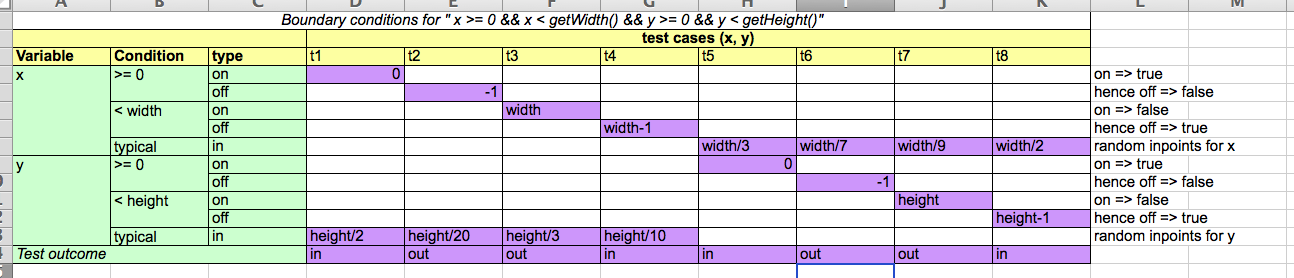
\includegraphics{3.3.9_domain_matrix.png}
\caption{Domain Matrix}
\end{figure}

\section{3.4 Understanding your tests}\label{understanding-your-tests}

\subsection{3.4.11}\label{section-6}

If the test methods in a class start with duplicate initialization code
this can be moved into a common initialization method with the @Before
annotation, because this method will be executed before every single
execution of a test method. Also, when a method needs to be tested using
multiple values as input (as in boundary testing for example),the test
can be parameterized, which prevents writing same pieces of code around
the input values.

\subsection{3.4.12}\label{section-7}

Using clean instances of the class under test, is necessary for
independence among tests. The impact that one test has on another should
be minimized to be sure that when a test fails, it only fails because of
that test.

\subsection{3.4.13}\label{section-8}

The difference between \texttt{assertTrue(a\ ==\ 1)} and
\texttt{assertEquals(a,\ 1)} is that the \texttt{assertEquals} gives a
comparison of the expected value with the actual value, whereas
\texttt{assertTrue} does not. So \texttt{assertEquals} is more useful,
as it provides information that can be used debug a failing test.

\subsection{3.4.14}\label{section-9}

One could make the argument that it is not necessary to test the private
methods of \texttt{MapParser} because all of the end-to-end tests rely
on a \texttt{Launcher} which makes use of \texttt{MapParser}. So, we
would expect a faulty \texttt{MapParser} to yield failing end-to-end
tests. However, it is also the case that a faulty \texttt{MapParser} may
make it difficult to debug the failing end-to-end tests, without having
isolated tests of the private methods of \texttt{MapParser} itself.
Furthermore, a passing test does necessarily not guarantee anything if
the test itself has faults. So, a passing end-to-end test does not
neceaarily guarantee that \texttt{MapParser} would not fail an isolated
test. In conclusion, it would probably be a good idea to test the
private methods in isolation.

\subsection{3.5}\label{section-10}

\subsubsection{3.5.15}\label{section-11}

There is one warning that remains in IntelliJ. IntelliJ complains that
\texttt{public\ class\ WithinBordersTest} can be private. We left this
public because the comment in \texttt{ParameterizedAssignment}
specifically states that it needs to be public.

In terms of the additional adequacy achieved thanks to our classes, we
measured the new overall coverage to be 89\%, with a line coverage of
84\%. So, our efforts have contributed 2 percentage points to the
overall line coverage, as compared to what we measured in question
3.1.1.

The continuous integration server confirmed that our builds worked
properly in most cases. We generally tried to avoid successively failing
builds on DevHub, as evidenced by the many green commits. We used Git
very extensively. In general, we tried to make new branches for
different exercises. This allowed us to divide the work effectively and
gives a very clear record of what was done.

\section{4.3 Testing Collisions}\label{testing-collisions}

\subsection{4.3.20}\label{section-12}

\begin{longtable}[]{@{}lllll@{}}
\toprule
& r1 & r2 & r3 & r4\tabularnewline
\midrule
\endhead
player & collider & collider & collidee &\tabularnewline
ghost & collidee & & collider & collider\tabularnewline
pellet & & collidee & & collidee\tabularnewline
& & & &\tabularnewline
outcome & player moves & player moves & ghost moves & ghost
moves\tabularnewline
& player dies & player earns points & player dies & pellet
remains\tabularnewline
& & pellet disappears & &\tabularnewline
& & & &\tabularnewline
\bottomrule
\end{longtable}

\subsection{4.3.24}\label{section-13}

\begin{longtable}[]{@{}lll@{}}
\toprule
& framework line coverage & our line coverage\tabularnewline
\midrule
\endhead
CollisionInteractionMap & 0\% & 94\%\tabularnewline
DefaultPlayerInteractionMap & 0\% & 100\%\tabularnewline
PlayerCollisions & 75\% & 79\%\tabularnewline
\bottomrule
\end{longtable}

Line coverage on PlayerCollisions have somewhat increases (4\%). The
original jpacman-framework did only cover collisions in which the player
was the collider. We covered collisions with a ghost as collider
aditionally.

The collision functionality that remains unchecked is the case when a
pellet is the collider. This however, is not a functionality that is
specified by the requirements and can therefore be left unchecked.

Also coverage on CollisionInteractionMap and DefaultPlayerInteractionMap
have increased drastically, only by applying the PlayerCollisions
testsuite on them too.

\section{4.4 Complex Tests}\label{complex-tests}

\subsubsection{4.4.25}\label{section-14}

It should not be the goal to achieve 100\% test coverage, because this
is very easily achieved by writing tests that are not meaningful.

An advantage of code coverage can be the ability to spot a decrease in
code coverage of a pull request.

A disadvantage is that high coverage can provide a false sense of
stability. 100\% coverage for example does not imply an absence of
faults.

\subsection{4.4.26}\label{section-15}

\texttt{LauncherSmokeTest.smokeTest()} can become flakey as a result of
an assumption that the call to \texttt{Thread.sleep(500L)} will be
sufficient to bring the monsters within 20 steps of the player. Since
the movement of the monsters depends on a random number generator, the
movements of the ghosts are not explicitly guaranteed to meet this
criterion. So, the call to
\texttt{assertThat(player.isAlive()).isFalse()} can sometimes yield a
failing test. The paper by Luo et al. identifies the three main causes
of flakey tests as (1) ``ASYNC WAIT'': asynchronous calls which do not
properly wait for the resource being called, (2) concurrency and (3)
test order dependency. Each type of flakey test has its own fix. For
example, for ASYNC WAIT, a common fix prescibed by Luo et al. is to
enforce the blocking of a given thread through \texttt{waitFor}. But,
the overarching theme of these fixes is that we need to enforce
determinism in our tests.

\subsubsection{4.4.27}\label{section-16}

A test that needs to communicate with infrastructure dependencies like a
database or http server will slow the entire test suite dramatically. To
mitigate this issue, you can mock these depencies and still test the
interaction.

\subsubsection{4.4.28}\label{section-17}

One disadvantage of using mocks is that one could make the mistake of
testing a mock by accident without realizing it. When using the more
advanced features of certain mocking frameworks there is a risk of
misunderstanding what exactly that code is doing, which may result in
green tests which don't actually test the software that is supposed to
be tested. Furthermore, the overextensive use of mocking can lead to
slower tests and possible problems that result from the interactions
between the mocks themselves.

\subsubsection{4.4.29}\label{section-18}

Mocking should mostly be done during unit testing, because it provides
isolation of the class under test. Mocking can be done during
integration testing for some dependencies that are not directly under
test. Mocking should not be done during system testing, because the
whole system should be under test and when using mocks, you are partly
testing your mocks instead of the real implementation.

\section{5.1 State Machines}\label{state-machines}

\subsection{5.1.31}\label{section-19}

\begin{figure}
\centering
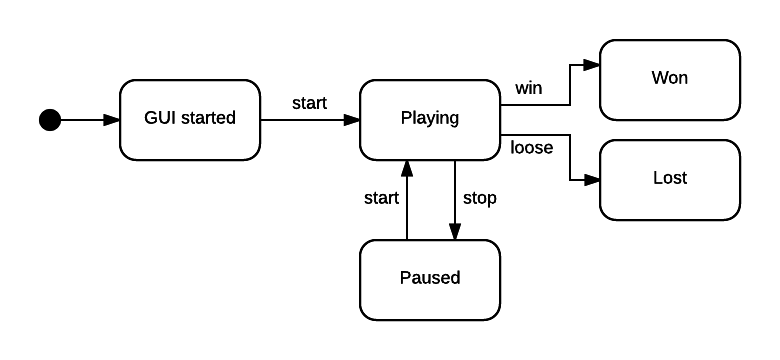
\includegraphics{5.1.31.png}
\caption{State Machine}
\end{figure}

\subsection{5.2.32}\label{section-20}

\begin{figure}
\centering
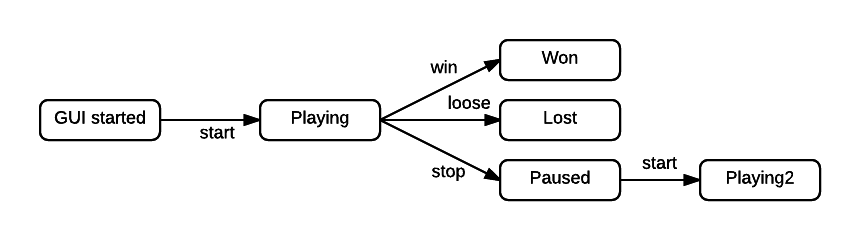
\includegraphics{5.1.32.png}
\caption{Transition Tree}
\end{figure}

\begin{longtable}[]{@{}llll@{}}
\toprule
Test Case ID & Start State & Events & End State\tabularnewline
\midrule
\endhead
T1 & GUI Started & start, win & Won\tabularnewline
T2 & GUI Started & start, loose & Lost\tabularnewline
T3 & GUI Started & start, stop, start & Playing\tabularnewline
\bottomrule
\end{longtable}

\subsection{5.2.33}\label{section-21}

\begin{longtable}[]{@{}lllll@{}}
\toprule
States & Events & & &\tabularnewline
\midrule
\endhead
& Stop & Start & Win & Lose\tabularnewline
& ----------- & ----------- & ------- & -------\tabularnewline
GUI Started & & Playing & &\tabularnewline
Playing & Paused & & Won & Lost\tabularnewline
Paused & & Playing & &\tabularnewline
\bottomrule
\end{longtable}

(state, event) pairs not contained in diagram:\\
(GUI Started, stop)\\
(GUI Started, win)\\
(GUI Started, loose)\\
(Playing, start)\\
(Paused, stop)\\
(Paused, win)\\
(Paused, loose)

\section{5.2 Multi-Level Games}\label{multi-level-games}

\subsection{5.2.37}\label{section-22}

\begin{figure}
\centering
\includegraphics{5.2.37.png}
\caption{Multilevel State Machine}
\end{figure}

\subsection{5.2.38}\label{section-23}

\begin{longtable}[]{@{}llll@{}}
\toprule
Test Case ID & Start State & Events & End State\tabularnewline
\midrule
\endhead
T1 & GUI Started & start, win level (\textless{}4) & Playing New
Level\tabularnewline
T2 & GUI Started & start, lose & Lost\tabularnewline
T3 & GUI Started & start, stop, start & Playing Level\tabularnewline
T4 & GUI Started & start, win level (=4) & Won Game\tabularnewline
\bottomrule
\end{longtable}

T2 and T3 could almost be reused, since they don't involve any change in
the level. But, it may still be necessary to modify them slightly, since
they should make use of the MultiGameLauncher, rather than the Launcher,
T1 would have to be modified further.

\section{5.3 Test Smells}\label{test-smells}

\subsection{5.3.46}\label{section-24}

Below, the \texttt{testWithinBorders} method has been changed to a
smelly multiple assertions test. Instead of being parameterized and
using a single \texttt{assertEquals}, the test now uses multiple asserts
and multiple types of asserts. Since \texttt{assertTrue} and
\texttt{assertFalse} don't give the expected and resulting values, it
would be difficult to determine why the test failed, since there are
multiple assertions that would give the same output on failure. In
contrast to this, the original, parameterized version of this test
allows us to identify specifically which input caused the test to fail.

\begin{verbatim}
@Test
    void testWithinBorders(int x, int y, boolean z) {
            int x = 0;
            int y = 3;
            assertTrue(board.withinBorders(x, y));
           `y = -1;
            assertFalse(board.withinBorders(x, y));
            y = -6;
            assertEquals(board.withinBorders(x, y), false);
            y = 0;
            x = -1;
            assertFalse(board.withinBorders(x, y));
            x = 3;
            assertThat(board.withinBorders(x, y)).isEqualTo(true);
            x = 1;
            assertTrue(board.withinBorders(x, y));
            x = 4;
            y = 2;
            assertEquals(board.withinBorders(x, y), false);
            x = 2;
            y = 5;
            assertTrue(board.withinBorders(x, y));
    }
\end{verbatim}

\subsection{5.3.47}\label{section-25}

Below, the \texttt{testAddSquareGround} method from the
\texttt{MapParserTest} class has been turned into an Irrelevant Details
test. In contrast to the original test method, the method below does not
use any mocks. As a result, the test could fail as a result of details
that are irrelevant to the method that we want to test. For example, the
improper implementation of BoardFactory, LevelFactory, and Square could
all cause the test to fail for reasons that have nothing to do with the
\texttt{addSquare} method that we wish to test. Futhermore, the use of
\texttt{asssertTrue} further obfuscates the results, since it does not
print the expected and actual values.

\begin{verbatim}
void testAddSquareGround() {
        Square grid = new Square(1,1);
        Square sq = new Square(1,1);
        grid[0][0] = null;
        BoardFactory bf = new BoardFactory();
        LevelFactory lf = new LevelFactory();
        MapParser mp = new MapParser(lf, bf);
        List<NPC> gh = new ArrayList<>();
        List<Square> = new ArrayList<>();

        mp.addSquare(gr, gh, sp, 0, 0, ' ');
        
        assertTrue(gr[0][0] == sq);

    }
\end{verbatim}

\section{5.5}\label{section-26}

\subsection{5.5.48}\label{section-27}

Three things that were good:

\begin{enumerate}
\def\labelenumi{\arabic{enumi}.}
\tightlist
\item
  Our test coverage has improved significantly since part 1. It would be
  very alarming if the opposite were true.
\item
  Our tests pass, which is always a good thing.
\item
  The JPacman Framework is a sufficiently complex piece of software such
  that the work of developing tests for it was varied, challenging, and
  interesting.
\end{enumerate}

Three things that were bad/annoying:

\begin{enumerate}
\def\labelenumi{\arabic{enumi}.}
\tightlist
\item
  The fact that DevHub could not handle the load/traffic at peak times
  (e.g.~right before the deadline) was problematic. It seems to suggest
  that DevHub has not been properly load tested. Perhaps this could be
  fixed by allocating more resources to DevHub during peak hours.
\item
  PMD/Checkstyle/Findbugs can be really annoying because they often
  complain about really stupid things and sometimes seem to complain
  about nonexistent issues. This can be fixed by either ignoring certain
  rules or by submitting bug reports (such as the TAs did in the case of
  PMD).
\item
  Mockito is not necessarily the best option for mocking. Its
  limitations, in terms of what it can or cannot mock or observe can be
  frustrating at times. A more powerful framework such as PowerMock
  might be a better alternative in the future.
\end{enumerate}

\end{document}
